\documentclass[conference]{IEEEtran}
\usepackage{cite}
\usepackage{amsmath,amssymb,amsfonts}
\usepackage{graphicx}
\usepackage{booktabs,tabularx,array,multirow}
\usepackage{algorithm}
\usepackage{algpseudocode}
\usepackage[hidelinks]{hyperref}
\newcolumntype{Y}{>{\raggedright\arraybackslash}X}

\begin{document}

\title{Lightweight Random Forest-Based Detection of Wi-Fi Evil Twin Attacks Using Beacon-Frame Fingerprints}

\author{\IEEEauthorblockN{Chawin Kitchat, Pannawat Thawonwong, and Somchart Fugkeaw}
\IEEEauthorblockA{School of Information, Computer and Communication Technology (ICT)\\
Sirindhorn International Institute of Technology, Thammasat University, Thailand\\
6622780227@g.siit.tu.ac.th, 662272372@g.siit.tu.ac.th, somchart@siit.tu.ac.th}}

\maketitle

\begin{abstract}
An Evil Twin access point imitates a legitimate Wi-Fi network to attract users and enable phishing, interception, or traffic manipulation. This paper presents a passive detector that classifies causal windows of IEEE 802.11 Beacon frames with a frozen Random Forest. The pipeline groups Beacons by claimed BSSID, constructs non-overlapping 20-Beacon windows, aggregates structural, security, physical-layer, temporal, and signal descriptors, and applies a fixed ensemble of 100 trees with maximum depth six. Development used chronological partitions of the public AWID3 Evil Twin capture. The selected preprocessing pipeline, model, and attack-probability threshold of 0.30 were frozen before evaluation on the separately collected D05-A-R2 capture. On the AWID3 temporal test block, the detector obtained 72 true positives and 86 true negatives, corresponding to an F1 score of 1.000. On D05-A-R2, it obtained 289 true positives, 489 true negatives, no false positives, and 72 false negatives, yielding precision 1.000, recall 0.801, F1 0.889, and balanced accuracy 0.900. Under the same W20 representation, CART, Logistic Regression, and K-nearest neighbors obtained F1 scores of 0.000, 0.000, and 0.033 on D05-A-R2; a causal sequence-five LSTM also obtained 0.000, although its support differs slightly. Detection-only Random Forest inference had P50, P95, and P99 single-window latencies of 15.99, 16.88, and 19.35 ms, and the serialized model occupied 126.2 KiB. These measurements support low per-decision latency and a compact model artifact, but not an embedded-memory claim because the isolated Python process reached 425.7 MiB peak RSS. The results demonstrate cross-dataset applicability to D05-A-R2 while also exposing limitations: AWID3 labels and temporal partitions originate from one capture, D05-A-R2 was previously inspected, and the experiment covers a limited set of AP hardware and attack conditions.
\end{abstract}

\begin{IEEEkeywords}
Evil Twin, Wi-Fi security, Beacon frames, Random Forest, AWID3, access-point fingerprinting, lightweight intrusion detection.
\end{IEEEkeywords}

\section{Introduction}

Wireless clients commonly identify a network by its service set identifier (SSID), even though the SSID is a public and configurable value. An adversary can advertise the same SSID as a legitimate access point (AP), copy visible security settings, and transmit a stronger signal to attract nearby clients. This impersonating device is commonly called an Evil Twin AP. Once a client associates with it, the attacker may display a captive portal, redirect traffic, observe inadequately protected communication, or place itself in a man-in-the-middle position. Because Beacon frames are broadcast before association and expose the configuration of an AP, they provide a practical source of evidence for early detection.

An Evil Twin detector faces a fundamental ambiguity. SSID, BSSID, security advertisements, supported rates, channel information, and many information elements (IEs) are not cryptographic identities. They may distinguish devices in a particular capture but remain copyable by an attacker. Received signal strength indicator (RSSI) values depend on location, transmit power, antenna orientation, and propagation. Timestamp and sequence behavior can be altered by resets, missed frames, or capture gaps. Consequently, a useful detector must be evaluated not only on a development dataset but also on observations collected with different hardware and under different environmental conditions.

Prior work has examined beacon fingerprinting, signal characteristics, clock skew, client-side path behavior, and machine-learning classifiers. ETGuard uses pre-association Beacon fingerprints and an enrolled database of legitimate APs~\cite{jain2019etguard}. Clock-skew approaches seek transmitter-specific timing characteristics~\cite{jana2010clock}, although their reliability against manipulation has been questioned~\cite{arackaparambil2010reliability}. Frame-classification research has reported promising results using compact selected attributes~\cite{asaduzzaman2020frames}. Machine-learning work using clock skew, RSSI, channel, and duration found Random Forest effective in its own ten-AP environment~\cite{seo2020reliability}. These studies establish that management frames contain discriminatory evidence, but their datasets, observation times, attack constructions, and prediction units differ. Reported percentages are therefore not directly interchangeable.

This study focuses on a deliberately simple final detector: a frozen Random Forest operating on causal 20-Beacon windows. The system is passive and does not associate with, probe, or transmit deauthentication frames toward observed networks. It parses Beacon observations from a packet capture (PCAP), groups them by the claimed BSSID, aggregates a fixed feature schema, and produces an attack probability for each completed window. A threshold of 0.30 maps the probability to either \emph{Normal} or \emph{Evil Twin Suspected}. No registry rule, Time-Shield decision, or other detector is fused into the final prediction. This separation makes the reported result attributable to the trained Random Forest alone.

The experimental design distinguishes internal discrimination from cross-dataset applicability. The public AWID3 Evil Twin capture~\cite{chatzoglou2021awid3} is divided chronologically for training, model selection, and internal testing. The independently collected D05-A-R2 capture is then used as a cross-dataset evaluation after freezing the model. The D05-A-R2 labels use the operator-confirmed roles of the two APs in the controlled capture: the Deco AP is legitimate and the Zyxel AP is the Evil Twin. Although the model was frozen before this evaluation, D05-A-R2 had been inspected in earlier project stages; it is therefore reported as a \emph{previously inspected cross-dataset test}, not an untouched independent test.

The contributions of this paper are as follows:
\begin{enumerate}
    \item an end-to-end RF-only pipeline from IEEE 802.11 Beacon frames to causal W20 predictions, using a deployment-compatible feature transformation and an explicit feature denylist;
    \item a chronological AWID3 development protocol with a frozen model, preprocessing pipeline, threshold, and reproducibility hashes;
    \item cross-dataset evaluation on D05-A-R2 with confusion counts, precision, recall, F1, balanced accuracy, and a comparison against CART, Logistic Regression, KNN, and a causal LSTM baseline; and
    \item a lightweight assessment that separates model artifact size and detection-only latency from the memory cost of the Python runtime.
\end{enumerate}

The remainder of this paper reviews related detection approaches, describes the detector and its feature construction, defines the evaluation protocol, presents the results, and discusses validity and deployment limitations.

\section{Related Work}

\subsection{Beacon and AP Fingerprinting}

Beacon fingerprinting attempts to identify inconsistencies between an observed AP and an expected profile. ETGuard constructs fingerprints from Beacon-frame fields and detects Evil Twins before client association~\cite{jain2019etguard}. It uses a client--server architecture and an incrementally maintained collection of legitimate fingerprints. The evaluation covers twelve attack scenarios and reports no false negatives and one false-positive scenario. ETGuard is an important comparison because it also uses passively visible management-frame information. However, it assumes an enrolled infrastructure, employs its own scenario-level evaluation, and does not use the AWID3-to-D05 transfer protocol of the present study. Its result is therefore discussed qualitatively rather than ranked numerically against our W20 F1 score.

RSSI has also been used as a fingerprint. Tang \emph{et al.} investigated RSSI-based Evil Twin detection in smart homes and reported detection success above 90\% under their studied conditions~\cite{tang2017rssi}. Signal evidence is attractive because a nearby attacker may have a noticeably different path to the receiver. At the same time, an RSSI value can encode the receiver position or attacker's transmit power rather than stable device identity. The present work includes signal summaries as features but does not interpret them as immutable fingerprints.

\subsection{Temporal and Client-Side Detection}

Jana and Kasera proposed detecting unauthorized APs using clock skew estimated from wireless timestamps~\cite{jana2010clock}. Clock behavior may distinguish oscillators even when advertised network identifiers match. Arackaparambil \emph{et al.} subsequently showed that clock-skew fingerprinting can be manipulated and evaluated methods for improving reliability~\cite{arackaparambil2010reliability}. These findings motivate including TSF progression and sequence continuity as model inputs while avoiding claims that timing alone proves physical identity.

Active client-side methods infer an additional wireless hop or a modified communication path. Yang \emph{et al.} proposed statistical techniques that do not require a preconfigured authorized-AP list~\cite{yang2012active}. Lu \emph{et al.} proposed a passive client-side technique based on statistical characteristics of 802.11 data frames and reported 96\% accuracy in their environment~\cite{lu2018etspotter}. Such methods observe forwarding behavior after or around client communication, whereas our detector operates only on Beacon windows and can produce a prediction before association. The difference in evidence and experimental unit prevents a direct accuracy comparison.

\subsection{Machine Learning for Evil Twin Detection}

Asaduzzaman \emph{et al.} evaluated frame classification and feature-selection methods for Evil Twin detection~\cite{asaduzzaman2020frames}. Their study reduced 38 initial attributes to ten and reported 91.2367\% accuracy for J48 on 5,911 captured instances. Seo \emph{et al.} compared Logistic Regression, Naive Bayes, KNN, support-vector machines, and Random Forest using clock skew, RSSI, channel, and duration~\cite{seo2020reliability}. Their Random Forest achieved approximately 99.5--100\% accuracy across the reported tests, with about a 1\% false-positive rate noted under environmental variation. Their detector required roughly 300--500 Beacons collected over ten minutes for a decision. In contrast, our prediction unit contains 20 Beacons, and the model is evaluated across two datasets rather than only within the authors' collection environment.

The AWID3 dataset was created to support evaluation of attacks against modern IEEE 802.11 enterprise networks, including Evil Twin and other wireless attacks~\cite{chatzoglou2021awid3}. Its PCAP representation permits independent feature extraction from original frames. Nevertheless, a temporal train/test split from one capture may remain easy because AP hardware, receiver placement, and firmware-specific advertisement patterns persist across partitions. This work therefore reports AWID3 as an internal temporal test and gives D05-A-R2 the primary role in assessing cross-dataset applicability.

\subsection{Positioning of This Work}

The proposed system does not claim a new Random Forest algorithm~\cite{breiman2001rf}. Its contribution is the reproducible construction and evaluation of an RF-only detector whose inputs are causal Beacon windows and whose cross-dataset behavior is reported without silently changing the threshold. Random Forest is selected because the frozen ensemble produced materially better D05-A-R2 recall than the evaluated CART, Logistic Regression, KNN, and LSTM baselines. The result is not presented as superiority over ETGuard or other papers because no common benchmark, packet membership, or label protocol exists.

\section{Our Proposed RF-Based Evil Twin Detection Approach}
\label{sec:system}

\subsection{System Model}

Fig.~\ref{fig:architecture} shows the final RF-only pipeline. Offline analysis begins with a PCAP containing IEEE 802.11 Beacon frames. The same feature path can also process chronologically delivered Beacon observations, but the current implementation and evaluation are offline post-processing rather than a live streaming deployment. Each valid Beacon is parsed into identity, capability, security, IE, radio, sequence, TSF, and timing fields. Observations are grouped by claimed BSSID and ordered causally. Every 20 consecutive Beacons form one non-overlapping window; incomplete tails are excluded from binary scoring.

\begin{figure*}[t]
    \centering
    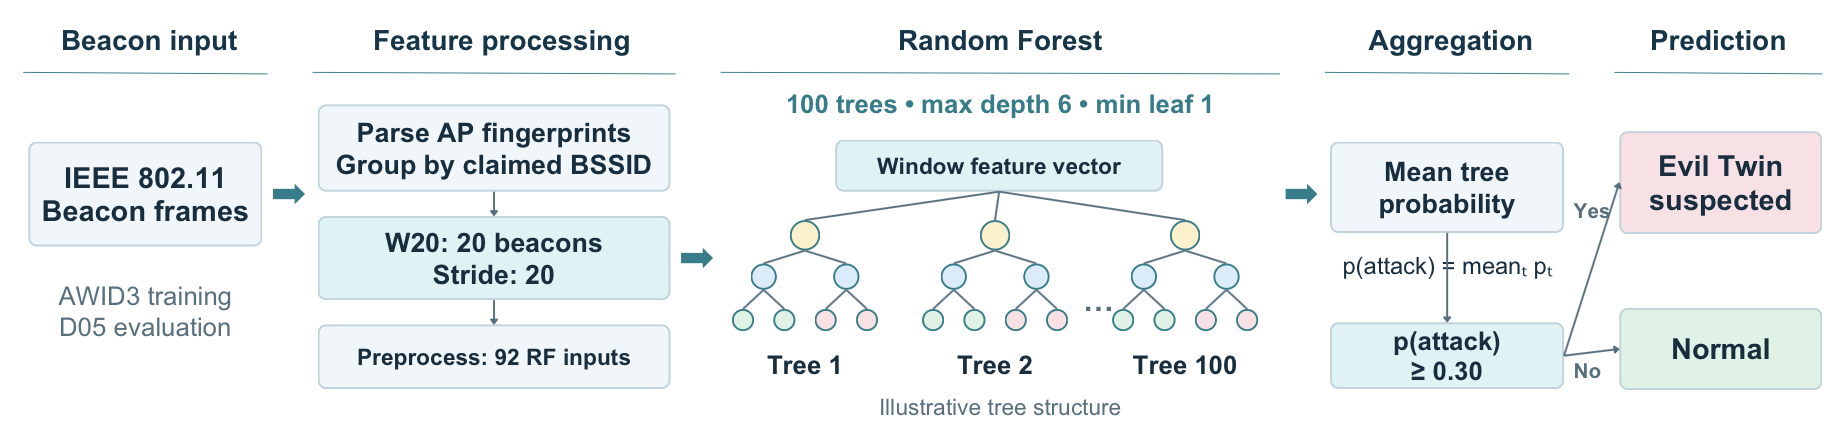
\includegraphics[width=0.98\textwidth,keepaspectratio]{Fig1.png}
    \caption{RF-only Evil Twin detection pipeline. Beacon observations are grouped by claimed BSSID, aggregated into causal non-overlapping W20 fingerprints, transformed to the frozen feature representation, evaluated by 100 decision trees, and thresholded at an attack probability of 0.30.}
    \label{fig:architecture}
\end{figure*}

The W20 row is passed to a serialized preprocessing pipeline and Random Forest. The preprocessing object was fitted only on the AWID3 training block. The ensemble outputs a probability by averaging the attack-class probabilities of its 100 trees. A probability at or above 0.30 is labeled \emph{Evil Twin Suspected}; a lower value is labeled \emph{Normal}. Both the probability and the binary decision are retained for audit.

\subsection{Beacon Parsing and Window Membership}

The extractor admits IEEE 802.11 Beacon frames and records the original source file, packet number, capture timestamp, claimed SSID and BSSID, capability bits, advertised Beacon interval, security IEs, supported rates, vendor IE summaries, PHY indicators, radiotap signal information when available, sequence-control values, retry flags, and TSF values. Malformed or unusable records do not silently become normal observations.

For a capture $c$ and claimed BSSID $b$, let the ordered Beacon sequence be
\begin{equation}
\mathcal{B}_{c,b}=\left(B_1,B_2,\ldots,B_n\right),
\end{equation}
where ordering follows the original packet sequence. Non-overlapping windows are
\begin{equation}
W_k=\left(B_{20k+1},\ldots,B_{20k+20}\right),
\label{eq:window}
\end{equation}
with a stride of 20. Grouping by claimed BSSID prevents frames from unrelated advertised identities from being combined. It does not prove that every frame with the same BSSID originates from the same physical radio. A SHA-256 membership hash derived from the ordered packet membership permits equivalence checks across evaluation implementations.

The W20 choice limits decision delay compared with methods requiring hundreds of Beacons while providing enough observations to calculate variability, continuity, and availability descriptors. Earlier AWID3 window-size experiments with W10, W20, and W50 all produced F1=1.000 on the internal validation data. W20 was frozen as the operational compromise before the D05-A-R2 result was used for final reporting; it was not reselected to improve that test.

\subsection{Feature Representation}

Each window produces a 96-column table row containing predictive descriptors and audit metadata. Seven forbidden metadata fields---BSSID, ordered frame membership, label purity, membership hash, source file, window start, and window end---are explicitly denied to the model. SSID and labels likewise do not enter the classifier. The frozen transformer produces 92 RF inputs: 84 numerical values, five missingness indicators, and three encoded categorical values. Table~\ref{tab:features} summarizes the major predictive families.

\begin{table*}[t]
\caption{Window-Level Feature Families Used by the Frozen Random Forest}
\label{tab:features}
\centering
\footnotesize
\begin{tabularx}{\textwidth}{@{}p{25mm}p{28mm}Y@{}}
\toprule
\textbf{Family} & \textbf{Examples} & \textbf{Window representation and rationale}\\
\midrule
Capability and structure & capability, ESS, privacy, preamble, slot, IE counts and lengths & Means and stability descriptors represent the advertised AP configuration and structural consistency of Beacon IEs.\\
Security & RSN, AKM, ciphers, PMF, RSNXE & Presence, stability, and change counts capture security-profile differences without using SSID or BSSID as predictors.\\
PHY and channel & VHT, HE, EHT, advertised channel, observed frequency & Presence states, stability, and changes summarize the advertised and receiver-observed radio configuration.\\
Vendor and WPS & vendor IE count, lengths, OUI/type diversity, WPS & Aggregate vendor descriptors retain structural information while avoiding a direct source identifier.\\
Temporal and sequence & duration, inter-arrival moments, TSF resets, sequence discontinuity, missing-Beacon estimate, retry rate & Causal window summaries measure timing and continuity without using absolute epoch time or raw packet index.\\
Signal and availability & RSSI moments and range; radiotap availability & Signal summaries provide environmental evidence; explicit availability fields prevent missing metadata from being confused with a valid zero.\\
\bottomrule
\end{tabularx}
\end{table*}

Numerical missing values are handled by the fitted imputation stage. Categorical values are encoded using training-fitted categories, with previously unseen levels handled by the declared preprocessing behavior. The model schema is serialized together with the classifier. This prevents an evaluation script from reordering features or refitting preprocessing on D05-A-R2.

\subsection{Frozen Random Forest Decision}

The selected classifier contains $T=100$ trees, maximum depth six, and minimum leaf size one. Balanced class weights were used during fitting. For a transformed W20 vector $\mathbf{x}_k$, tree $t$ produces an attack probability $p_t(1\mid\mathbf{x}_k)$. The ensemble probability is
\begin{equation}
p_{\mathrm{attack}}(\mathbf{x}_k)=\frac{1}{T}\sum_{t=1}^{T}p_t(1\mid\mathbf{x}_k).
\label{eq:rfprob}
\end{equation}
The binary prediction is
\begin{equation}
\hat{y}_k=\begin{cases}
1,&p_{\mathrm{attack}}(\mathbf{x}_k)\geq 0.30,\\
0,&p_{\mathrm{attack}}(\mathbf{x}_k)<0.30.
\end{cases}
\label{eq:threshold}
\end{equation}
The threshold was selected using the AWID3 validation block together with the designated D02 legitimate-only calibration capture. D05-A-R2 was not used to refit the classifier, preprocessing pipeline, or threshold. The final model SHA-256 is \texttt{8a1e1717f77ded865\allowbreak{}336c7d4d9c3db815\allowbreak{}59bb1300cb979e73\allowbreak{}c803f02f26ed145}.

Algorithm~\ref{alg:detection} summarizes causal inference. The algorithm never reads a ground-truth label during prediction; labels are joined only after output generation to calculate evaluation metrics.

\begin{algorithm}[t]
\caption{Causal RF-Only W20 Detection}
\label{alg:detection}
\begin{algorithmic}[1]
\Require Ordered Beacon observations, frozen transformer $g$, frozen forest $\mathcal{F}$, threshold $\tau=0.30$
\Ensure Per-window probability and prediction
\State Group observations by capture and claimed BSSID
\For{each group in chronological order}
    \State Partition into complete non-overlapping windows of 20 Beacons
    \For{each window $W_k$}
        \State Compute deployment-eligible descriptors $\mathbf{f}_k$
        \State Remove identity, provenance, time-boundary, and label fields
        \State $\mathbf{x}_k \gets g(\mathbf{f}_k)$
        \State $p_k \gets \frac{1}{100}\sum_{t=1}^{100}p_t(1\mid\mathbf{x}_k)$
        \State $\hat y_k \gets \mathbb{1}[p_k\geq\tau]$
        \State Emit membership hash, window time, $p_k$, and $\hat y_k$
    \EndFor
\EndFor
\end{algorithmic}
\end{algorithm}

\subsection{Threat Model and Scope}

The attacker may create a competing AP, copy SSID and BSSID values, reproduce visible security and capability fields, choose a channel, and modify transmit power. The receiver is trusted, and the attacker is not assumed to alter the stored model or evaluation files. The detector targets observable differences in Beacon-window fingerprints; it does not cryptographically authenticate the transmitter. An attacker that precisely reproduces all learned descriptors may evade detection. Conversely, a legitimate AP whose hardware or firmware resembles the AWID3 attack profile may be misclassified. The output phrase \emph{Evil Twin Suspected} reflects this evidentiary limit.

\section{Experiment Setup}
\label{sec:method}

\subsection{Dataset Roles and Ground Truth}

Table~\ref{tab:datasets} defines the only two datasets used for the main performance claims. The AWID3 Evil Twin PCAP is the public development source. Its original file SHA-256 is \texttt{a3fbdf8368d7ced3\allowbreak{}83829540d2dd6240\allowbreak{}73847c60411fa393\allowbreak{}4ea647446bda43a8}. The project applies the documented AWID3 attack rule and constructs profile-level W20 labels. These are dataset-derived attack/normal proxy labels, not independent physical-transmitter attestation. This distinction matters because a high internal score may reflect persistent device and capture characteristics.

D05-A-R2 is a controlled capture collected with a legitimate Deco AP and a Zyxel AP operating as the Evil Twin. The protected SSID is \texttt{pandee}; the operator-confirmed legitimate Deco BSSID is \texttt{ba:a7:b9:ae:39:1c}, and the controlled Evil Twin Zyxel BSSID is \texttt{28:28:5d:a6:1c:28}. Other ambient APs are excluded from labeled metrics. The capture begins at 21:24:14.906661, and the first observed Zyxel Beacon occurs at 21:29:13.411338. Ground truth is assigned by the controlled AP role, not supplied to the model.

\begin{table*}[t]
\caption{Dataset Roles in the Final RF-Only Evaluation}
\label{tab:datasets}
\centering
\footnotesize
\begin{tabularx}{\textwidth}{@{}p{23mm}p{26mm}p{32mm}Y@{}}
\toprule
\textbf{Dataset} & \textbf{Role} & \textbf{Prediction unit} & \textbf{Ground-truth and validity statement}\\
\midrule
AWID3 Evil Twin & Training, validation, internal temporal test & Profile W20, stride 20 & Dataset-derived proxy labels from one original capture. Temporal separation reduces immediate adjacency leakage but does not establish new-device independence.\\
D05-A-R2 & Cross-dataset evaluation & Identity W20, stride 20 & Controlled AP-role labels: Deco legitimate and Zyxel Evil Twin. Ambient APs excluded. Model frozen before evaluation, but the capture was previously inspected during the wider project.\\
\bottomrule
\end{tabularx}
\end{table*}

\subsection{Chronological Development and Freeze Protocol}

The AWID3 W20 table is split chronologically using 60\% of the capture duration for training, the next 20\% for validation, and the final 20\% for internal testing. Windows crossing temporal boundaries are excluded. The resulting internal test contains 158 windows: 86 dataset-derived normal windows and 72 attack windows. Chronological splitting is preferred to random row splitting because neighboring Beacon windows from the same episode are highly correlated. It does not, however, eliminate dependence on the same receiver, AP profiles, and capture session.

Model-family candidates and thresholds are evaluated only on development data. The final RF configuration uses 100 trees, maximum depth six, minimum leaf size one, and threshold 0.30. The serialized preprocessing and classifier are frozen before producing D05-A-R2 predictions. Freeze metadata records the model hash, seed 20261116, training source, schema, selected threshold, and declared development datasets. Evaluation code checks the hash and threshold before inference.

The final choice of RF as the paper's detector occurred after multiple project experiments, including inspection of D05 behavior. Therefore, the model was technically frozen before D05-A-R2 inference, but the final research narrative must not present D05-A-R2 as a pristine model-selection-independent test. We use the more precise term \emph{previously inspected cross-dataset evaluation}.

\subsection{Baseline Models}

Four baselines are compared. CART uses maximum depth three, minimum leaf size five, and threshold 0.30. Logistic Regression uses $C=0.1$, balanced class weighting, training-fitted scaling, and threshold 0.30. KNN uses five neighbors, uniform weighting, Euclidean distance, training-fitted numerical preprocessing, and threshold 0.50. These three baselines and RF produce one prediction for every eligible W20 window.

The LSTM uses hidden size eight and consumes causal sequences of five W20 vectors. It cannot predict the first four windows of each capture/BSSID group without padding, so its support is slightly smaller: 150 AWID3 temporal-test decisions and 842 D05-A-R2 decisions. LSTM results are included as a sequence-model diagnostic and are marked as not strictly identical in prediction support. Hyperparameters and thresholds were selected using AWID3 validation only; no baseline was tuned from D05-A-R2 outcomes.

\subsection{Metrics}

For the Evil Twin positive class, true positives (TP) and false negatives (FN) are attack windows predicted as attack and normal, respectively. True negatives (TN) and false positives (FP) are legitimate windows predicted as normal and attack. We report
\begin{align}
\mathrm{Precision} &= \frac{TP}{TP+FP},\\
\mathrm{Recall} &= \frac{TP}{TP+FN},\\
F_1 &= \frac{2\,\mathrm{Precision}\,\mathrm{Recall}}
{\mathrm{Precision}+\mathrm{Recall}},\\
\mathrm{FPR} &= \frac{FP}{FP+TN},\\
\mathrm{Balanced\ Accuracy} &= \frac{1}{2}\left(\frac{TP}{TP+FN}+\frac{TN}{TN+FP}\right).
\end{align}
Confusion counts are reported because F1 alone can hide whether a detector misses attacks or over-alerts on legitimate windows.

\subsection{Lightweight Measurement}

Detection-only timing uses pre-extracted W20 inputs so that repeated PCAP decoding does not dominate inference measurements. One warm-up repetition precedes five measured repetitions. Each single-window call includes the frozen preprocessing pipeline and RF probability calculation. Latency percentiles, CPU time, throughput, Python incremental allocation, isolated-process peak RSS, and serialized model size are recorded on the same machine and Python environment. Beacon-level parsing and W20 detection are not compared as if they were the same prediction unit.

The computational workload is not reused to create new detection-performance claims. Model performance is calculated only from the labeled AWID3 and D05-A-R2 windows, while timing describes the cost of executing the detector.

\section{Evaluation}
\label{sec:results}

\subsection{Frozen Random Forest Performance}

Table~\ref{tab:rfresults} presents the main RF results. The AWID3 internal temporal test is perfectly separated: all 72 attack windows and 86 dataset-derived normal windows are classified correctly. Because all windows originate from the same public capture used for development, this result demonstrates within-capture temporal discrimination rather than independent-device generalization.

On D05-A-R2, the frozen RF classifies all 489 legitimate Deco windows as normal. It detects 289 of 361 Evil Twin Zyxel windows and misses 72. Precision is therefore 1.000, recall is 0.801, F1 is 0.889, and balanced accuracy is 0.900. The absence of false positives in this capture should not be generalized to arbitrary legitimate APs; it is a result for the controlled D05-A-R2 scope.

\begin{table}[t]
\caption{Frozen Random Forest Performance}
\label{tab:rfresults}
\centering
\footnotesize
\begin{tabular}{@{}lrrrrrr@{}}
\toprule
\textbf{Dataset} & \textbf{TN} & \textbf{FP} & \textbf{FN} & \textbf{TP} & \textbf{Recall} & \textbf{$F_1$}\\
\midrule
AWID3 test & 86 & 0 & 0 & 72 & 1.000 & 1.000\\
D05-A-R2 & 489 & 0 & 72 & 289 & 0.801 & 0.889\\
\bottomrule
\end{tabular}
\end{table}

The D05-A-R2 confusion matrix reveals the practical trade-off at the frozen threshold. The detector is conservative in this capture: it never flags the legitimate Deco AP, but it leaves 19.9\% of the Evil Twin windows undetected. Because each W20 decision represents a completed 20-Beacon group, FN values indicate intervals without an alert rather than 72 distinct attackers. An operator interpreting these predictions should use window-level evidence and alert timing rather than treating every positive window as an independent incident.

\subsection{Comparison with Baseline Models}

Table~\ref{tab:baselines} compares model families. RF, CART, Logistic Regression, and KNN use the same W20 support. LSTM uses causal sequences of five windows and consequently has eight fewer D05-A-R2 decisions and eight fewer AWID3 decisions.

\begin{table*}[t]
\caption{Model Comparison on AWID3 Temporal Test and D05-A-R2}
\label{tab:baselines}
\centering
\footnotesize
\begin{tabular}{@{}llrrrrrrrr@{}}
\toprule
\textbf{Dataset} & \textbf{Model} & \textbf{$N$} & \textbf{TN} & \textbf{FP} & \textbf{FN} & \textbf{TP} & \textbf{Precision} & \textbf{Recall} & \textbf{$F_1$}\\
\midrule
\multirow{5}{*}{AWID3 test}
 & Frozen RF & 158 & 86 & 0 & 0 & 72 & 1.000 & 1.000 & 1.000\\
 & CART & 158 & 86 & 0 & 72 & 0 & 0.000 & 0.000 & 0.000\\
 & Logistic Regression & 158 & 86 & 0 & 0 & 72 & 1.000 & 1.000 & 1.000\\
 & KNN & 158 & 86 & 0 & 0 & 72 & 1.000 & 1.000 & 1.000\\
 & LSTM (Seq5) & 150 & 82 & 0 & 0 & 68 & 1.000 & 1.000 & 1.000\\
\midrule
\multirow{5}{*}{D05-A-R2}
 & Frozen RF & 850 & 489 & 0 & 72 & 289 & 1.000 & 0.801 & 0.889\\
 & CART & 850 & 0 & 489 & 361 & 0 & 0.000 & 0.000 & 0.000\\
 & Logistic Regression & 850 & 489 & 0 & 361 & 0 & 0.000 & 0.000 & 0.000\\
 & KNN & 850 & 489 & 0 & 355 & 6 & 1.000 & 0.017 & 0.033\\
 & LSTM (Seq5) & 842 & 485 & 0 & 357 & 0 & 0.000 & 0.000 & 0.000\\
\bottomrule
\end{tabular}
\end{table*}

The internal AWID3 result alone does not identify a robust model. Logistic Regression, KNN, LSTM, and RF all obtain F1=1.000, while CART predicts no AWID3 test attacks under its validation-selected configuration. The cross-dataset result separates the candidates more clearly. Logistic Regression and LSTM predict every D05-A-R2 attack window as normal. KNN detects only six of 361 attack windows. CART performs worse: it flags all 489 legitimate windows while missing all 361 attack windows. RF is the only evaluated model that retains substantial attack recall while preserving zero false positives in D05-A-R2.

These failures illustrate why an internal perfect score is insufficient. A linear separator or neighborhood relationship that fits one capture may not survive changes in AP hardware and receiver conditions. The shallow CART's reversed behavior on D05-A-R2 is particularly consistent with a shortcut boundary that does not transfer. The RF ensemble does not eliminate domain shift, as shown by its 72 false negatives, but it provides the best observed balance among the evaluated candidates.

\subsection{Lightweight Results}

Table~\ref{tab:lightweight} reports detection-only measurements for the frozen RF. The serialized artifact is 129,244 bytes (126.2 KiB). Median single-window latency is 15.99 ms, with P95 and P99 below 20 ms. Throughput is 62.8 W20 decisions/s under repeated single-window calls. Because a decision consumes 20 Beacons, this computational rate is substantially faster than the arrival rate of a single normally beaconing AP. Actual multi-AP capacity also depends on decoding, feature extraction, operating-system scheduling, and batching.

\begin{table}[t]
\caption{Frozen RF Detection-Only Cost per W20}
\label{tab:lightweight}
\centering
\footnotesize
\begin{tabular}{@{}lr@{}}
\toprule
\textbf{Measurement} & \textbf{Result}\\
\midrule
Model artifact & 126.2 KiB\\
Latency P50 & 15.99 ms\\
Latency P95 & 16.88 ms\\
Latency P99 & 19.35 ms\\
CPU time/window & 10.55 ms\\
Throughput & 62.8 W20/s\\
Python incremental peak & 4.21 MiB\\
Isolated process peak RSS & 425.7 MiB\\
\bottomrule
\end{tabular}
\end{table}

The measurements support two narrow lightweight claims. First, the learned artifact is compact. Second, per-window inference latency is small relative to the time needed to collect 20 Beacon frames. They do not support a general claim that the complete Python application is memory-light: isolated process peak RSS includes the interpreter, scientific libraries, model runtime, and loaded data, and reaches 425.7 MiB. Embedded deployment would require measurement on the intended hardware and likely a reduced runtime or exported model representation.

\subsection{Window Size and Decision Delay}

The earlier AWID3 window experiment evaluated W10, W20, and W50 with non-overlapping strides. All three achieved F1=1.000 on the corresponding within-capture validation windows. This tie means the AWID3 score cannot justify choosing a larger window. W20 was retained because it provides twice the observations of W10 for stability descriptors while requiring fewer Beacons than W50. At a nominal 100 TU Beacon interval, 20 Beacons correspond to roughly two seconds of observation, although missed frames, channel scanning, and contention can increase wall-clock delay. The paper reports this as an approximate collection delay, not a measured live alert latency.

\subsection{Discussion}

\subsubsection{What the Results Establish}

The primary empirical finding is that the RF learned from AWID3 transfers partially to D05-A-R2. The two datasets differ in AP identities and capture conditions, yet the frozen model detects 80.1\% of the controlled Evil Twin windows with no false positives among the 489 legitimate windows in that capture. This result is stronger evidence of applicability than the perfect AWID3 temporal score because the latter retains the same capture and device profiles across partitions.

The baseline comparison also supports choosing RF as the final model among the evaluated candidates. Logistic Regression, KNN, and LSTM appear perfect on AWID3 but provide little or no attack recall on D05-A-R2. RF's ensemble can combine multiple nonlinear feature relationships rather than rely on one global linear boundary or local distance structure. However, the experiment does not establish that Random Forest is universally superior. It establishes only that this frozen RF outperformed these specific validation-selected baselines on the defined AWID3 and D05-A-R2 protocols.

\subsubsection{Interpretation of the False Negatives}

The 72 D05-A-R2 false negatives show that the detector does not identify every attack window. Some Evil Twin windows may resemble the AWID3-derived normal region in the transformed feature space, particularly when security and advertisement settings are deliberately matched. Environmental and hardware differences can shift both normal and attack distributions. Since the classifier operates independently on each W20, it does not accumulate evidence across several low-probability windows. A future study may evaluate calibrated persistence or domain adaptation, but doing so on D05-A-R2 after inspecting its errors would turn the test into development data. No such tuning is performed here.

The zero false positives should also be interpreted at the capture level. It means the RF did not flag any legitimate Deco W20 in D05-A-R2. It does not prove a zero false-positive rate for other legitimate vendors, firmware versions, channels, receiver locations, or operational changes. A broader prospective collection is necessary before deployment claims can be made.

\subsubsection{Relation to Prior Work}

The 0.889 D05-A-R2 F1 score must not be compared as a ranking against the accuracy values reported by ETGuard, ET-spotter, Asaduzzaman \emph{et al.}, or Seo \emph{et al.} ETGuard uses enrolled Beacon fingerprints and scenario-level outcomes~\cite{jain2019etguard}. ET-spotter uses data-frame forwarding characteristics~\cite{lu2018etspotter}. Asaduzzaman \emph{et al.} use their own frame instances and cross-validation~\cite{asaduzzaman2020frames}. Seo \emph{et al.} use 10-minute samples from ten APs and tune algorithm thresholds in their collection environment~\cite{seo2020reliability}. The present study uses W20 predictions, AWID3 development, and a controlled cross-dataset capture. A fair superiority claim would require executing competing implementations on identical packet membership and ground truth.

Our result complements rather than replaces these approaches. A registry-based fingerprint detector may provide strong authorization evidence where trusted enrollment is available. Traffic-path techniques may detect relaying behavior that Beacon features cannot expose. The RF-only design is attractive when only passively captured Beacons and a learned model are available, but it remains statistical rather than authoritative.

\subsubsection{Meaning of Lightweight}

The term \emph{lightweight} is often used ambiguously. In this paper it refers to a compact serialized RF artifact, bounded tree depth, causal fixed-size inputs, and low measured detection-only latency. It does not imply that PCAP decoding is free, that feature extraction consumes no memory, or that a Python scientific stack fits an embedded microcontroller. Reporting P50/P95/P99 latency and peak RSS prevents the small artifact size from being mistaken for the total application footprint.

The system is also operationally lightweight in that it does not associate with an AP, inject packets, alter the protocol, or require an active client flow. These properties reduce deployment interference. They do not resolve the need for a monitor-mode radio, channel coverage, sufficient Beacon capture quality, and secure handling of output alerts.

\subsection{Threats to Validity}

\subsubsection{Label Validity}

AWID3 provides the public attack capture and documented attack context, but the constructed normal/attack window labels are dataset-derived proxies. Frames outside an attack filter are not equivalent to independent proof of a legitimate physical transmitter. The AWID3 confusion matrix should therefore be read as agreement with the project's derived label protocol. D05-A-R2 has stronger operator-confirmed AP roles in a controlled experiment, but it still represents only one legitimate AP family and one attack AP family.

\subsubsection{Selection and Inspection Bias}

The model artifact was frozen before the reported D05-A-R2 inference and was not retrained or threshold-adjusted from that capture. Nevertheless, D05-A-R2 had been inspected during earlier phases of the project, and the final decision to present RF alone was made after observing multiple model results. This creates selection bias at the research-narrative level. The result is therefore cross-dataset but not an untouched independent confirmation. A future final test must be collected prospectively after freezing the RF-only protocol and paper hypotheses.

\subsubsection{Domain and Hardware Coverage}

The evaluation does not cover a broad range of vendors, receiver locations, channels, firmware updates, transmit powers, or deliberate feature-cloning strategies. The model may learn correlations specific to AWID3 and the tested APs. A same-SSID or same-BSSID claim alone is not evidence of a physical Evil Twin. The model is vulnerable to concept drift and to attackers that reproduce the learned feature distribution.

\subsubsection{Baseline Comparability}

RF, CART, Logistic Regression, and KNN share W20 support, but LSTM requires five-window sequences and excludes the first four windows per group. The LSTM row is therefore informative but not strictly identical in support. None of the external paper results are directly comparable because their datasets and units differ. This paper avoids claiming superiority over those systems.

\subsubsection{Computational Validity}

Timing measurements come from one hardware and software environment. Single-window calls may understate the throughput available from batching, while loaded-data RSS may overstate the footprint of a production service. End-to-end delay also includes Beacon collection, PCAP decoding, and feature extraction. The reported benchmark isolates detection cost and labels its scope accordingly.

\subsection{Reproducibility and Ethical Use}

The experiment preserves the original PCAP provenance, ordered W20 membership, model metadata, preprocessing schema, threshold, and SHA-256 hashes. The RF-only research package is regenerated with \texttt{.venv/bin/python scripts/build\_rf\_research\_package.py}, and the repository test suite is executed with \texttt{.venv/bin/pytest -q}. The completed suite contains 208 tests. Regeneration verifies the frozen RF hash and writes CSV tables for per-scenario performance, baseline comparison, lightweight measurements, window-size results, and literature positioning. Predictions are computed from features; confusion counts and plots are generated from the actual prediction artifacts rather than hard-coded result labels.

The detector is intended for authorized monitoring of networks and captures that the operator is permitted to inspect. The work does not require transmitting deauthentication frames or disrupting clients. Dataset handling should avoid collecting unrelated user traffic where Beacon-only capture is sufficient. Alerts should be reviewed as statistical evidence and not used as sole proof of malicious intent.

\section{Conclusion}

This paper presented a passive RF-only Evil Twin detector operating on causal, non-overlapping 20-Beacon fingerprints. The final model uses 100 depth-limited trees and a frozen attack threshold of 0.30. It achieved F1=1.000 on an AWID3 temporal test and F1=0.889 on the previously inspected D05-A-R2 cross-dataset evaluation, detecting 289 of 361 Evil Twin windows without flagging the 489 legitimate windows in that capture. CART, Logistic Regression, KNN, and LSTM did not retain comparable D05-A-R2 recall, despite several obtaining perfect AWID3 scores. This contrast demonstrates the importance of cross-dataset evaluation.

The 126.2 KiB model and approximately 16 ms median W20 inference latency support a compact and low-latency characterization. The 425.7 MiB isolated Python peak RSS prevents a broader embedded-memory claim. Most importantly, the results are limited by one AWID3 development capture, one controlled external capture, previously inspected test data, and narrow AP diversity. The next valid step is a prospective evaluation on newly collected legitimate and Evil Twin sessions after freezing the RF-only protocol, without changing features or threshold from the observed outcomes.

\begin{thebibliography}{00}

\bibitem{chatzoglou2021awid3}
E. Chatzoglou, G. Kambourakis, and C. Kolias, ``Empirical evaluation of attacks against IEEE 802.11 enterprise networks: The AWID3 dataset,'' \emph{IEEE Access}, vol. 9, pp. 34188--34205, 2021, doi: 10.1109/ACCESS.2021.3061609.

\bibitem{jain2019etguard}
V. Jain, V. Laxmi, M. S. Gaur, and M. Mosbah, ``ETGuard: Detecting D2D attacks using wireless evil twins,'' \emph{Computers \& Security}, vol. 83, pp. 389--405, 2019, doi: 10.1016/j.cose.2019.02.014.

\bibitem{jana2010clock}
S. Jana and S. K. Kasera, ``On fast and accurate detection of unauthorized wireless access points using clock skews,'' \emph{IEEE Trans. Mobile Comput.}, vol. 9, no. 3, pp. 449--462, 2010, doi: 10.1109/TMC.2009.145.

\bibitem{arackaparambil2010reliability}
C. Arackaparambil, S. Bratus, A. Shubina, and D. Kotz, ``On the reliability of wireless fingerprinting using clock skews,'' in \emph{Proc. ACM Conf. Wireless Network Security (WiSec)}, 2010, pp. 169--174, doi: 10.1145/1741866.1741894.

\bibitem{yang2012active}
C. Yang, Y. Song, and G. Gu, ``Active user-side evil twin access point detection using statistical techniques,'' \emph{IEEE Trans. Inf. Forensics Security}, vol. 7, no. 5, pp. 1638--1651, 2012, doi: 10.1109/TIFS.2012.2207383.

\bibitem{lu2018etspotter}
Q. Lu, H. Qu, Y. Zhuang, X.-J. Lin, and Y. Ouyang, ``Client-side evil twin attacks detection using statistical characteristics of 802.11 data frames,'' \emph{IEICE Trans. Inf. Syst.}, vol. E101-D, no. 10, pp. 2465--2473, 2018, doi: 10.1587/transinf.2018EDP7030.

\bibitem{asaduzzaman2020frames}
M. Asaduzzaman, M. S. Majib, and M. M. Rahman, ``Wi-Fi frame classification and feature selection analysis in detecting evil twin attack,'' in \emph{Proc. IEEE Region 10 Symposium (TENSYMP)}, 2020, pp. 1704--1707, doi: 10.1109/TENSYMP50017.2020.9231042.

\bibitem{seo2020reliability}
J. Seo, C. Cho, and Y. Won, ``Enhancing the reliability of Wi-Fi network using evil twin AP detection method based on machine learning,'' \emph{J. Inf. Process. Syst.}, vol. 16, no. 3, pp. 541--556, 2020, doi: 10.3745/JIPS.03.0137.

\bibitem{tang2017rssi}
Z. Tang, Y. Zhao, L. Yang, S. Qi, D. Fang, X. Chen, X. Gong, and Z. Wang, ``Exploiting wireless received signal strength indicators to detect evil-twin attacks in smart homes,'' \emph{Mobile Information Systems}, vol. 2017, Art. no. 1248578, 2017, doi: 10.1155/2017/1248578.

\bibitem{breiman2001rf}
L. Breiman, ``Random forests,'' \emph{Machine Learning}, vol. 45, pp. 5--32, 2001, doi: 10.1023/A:1010933404324.

\end{thebibliography}

\end{document}
